% The document class supplies options to control rendering of some standard
% features in the result.  The goal is for uniform style, so some attention 
% to detail is *vital* with all fields.  Each field (i.e., text inside the
% curly braces below, so the MEng text inside {MEng} for instance) should 
% take into account the following:
%
% - author name       should be formatted as "FirstName LastName"
%   (not "Initial LastName" for example),
% - supervisor name   should be formatted as "Title FirstName LastName"
%   (where Title is "Dr." or "Prof." for example),
% - degree programme  should be "BSc", "MEng", "MSci", "MSc" or "PhD",
% - dissertation title should be correctly capitalised (plus you can have
%   an optional sub-title if appropriate, or leave this field blank),
% - dissertation type should be formatted as one of the following:
%   * for the MEng degree programme either "enterprise" or "research" to
%     reflect the stream,
%   * for the MSc  degree programme "$X/Y/Z$" for a project deemed to be
%     X%, Y% and Z% of type I, II and III.
% - year              should be formatted as a 4-digit year of submission
%   (so 2014 rather than the accademic year, say 2013/14 say).


\documentclass[ % the name of the author
                    author={Callum Pearce},
                % the name of the supervisor
                supervisor={Dr. Neill Campbell},
                % the degree programme
                    degree={MEng},
                % the dissertation    title (which cannot be blank)
                     title={Learning the incident radiance for a continuous state space rather than a discrete one is more beneficial for Importance Sampling in Monte Carlo Path tracing},
                % the dissertation subtitle (which can be blank)
                  subtitle={},
                % the dissertation     type
                      type={research},
                % the year of submission
                      year={2019} ]{dissertation}

\begin{document}

% =============================================================================

% This section simply introduces the structural guidelines.  It can clearly
% be deleted (or commented out) if you use the file as a template for your
% own dissertation: everything following it is in the correct order to use 
% as is.
\begin{comment}
\section*{Prelude}
\thispagestyle{empty}

A typical dissertation will be structured according to (somewhat) standard 
sections, described in what follows.  However, it is hard and perhaps even 
counter-productive to generalise: the goal is {\em not} to be prescriptive, 
but simply to act as a guideline.  In particular, each page count given is
important but {\em not} absolute: their aim is simply to highlight that a 
clear, concise description is better than a rambling alternative that makes
it hard to separate important content and facts from trivia.

You can use this document as a \LaTeX-based~\cite{latexbook1,latexbook2} 
template for your own dissertation by simply deleting extraneous sections
and content; keep in mind that the associated {\tt Makefile} could be of
use, in particular because it automatically executes  to 
deal with the associated bibliography.  

You can, on the other hand, opt {\em not} to use this template; this is a 
perfectly acceptable approach.  Note that a standard cover and declaration 
of authorship may still be produced online via
\[
\mbox{\url{http://www.cs.bris.ac.uk/Teaching/Resources/cover.html}}
\]
\end{comment}

% =============================================================================

% This macro creates the standard UoB title page by using information drawn
% from the document class (meaning it is vital you select the correct degree 
% title and so on).

\maketitle

% After the title page (which is a special case in that it is not numbered)
% comes the front matter or preliminaries; this macro signals the start of
% such content, meaning the pages are numbered with Roman numerals.

\frontmatter

% This macro creates the standard UoB declaration; on the printed hard-copy,
% this must be physically signed by the author in the space indicated.

\makedecl

% LaTeX automatically generates a table of contents, plus associated lists 
% of figures, tables and algorithms.  The former is a compulsory part of the
% dissertation, but if you do not require the latter they can be suppressed
% by simply commenting out the associated macro.

\tableofcontents
% The following sections are part of the front matter, but are not generated
% automatically by LaTeX; the use of \chapter* means they are not numbered.

% -----------------------------------------------------------------------------

\subfile{chapters/executive_summary}

\subfile{chapters/supporting_technologies}

\subfile{chapters/notation_acronyms}

\subfile{chapters/acknowledgements}

% =============================================================================

% After the front matter comes a number of chapters; under each chapter,
% sections, subsections and even subsubsections are permissible.  The
% pages in this part are numbered with Arabic numerals.  Note that:
%
% - A reference point can be marked using \label{XXX}, and then later
%   referred to via \ref{XXX}; for example Chapter\ref{chap:context}.
% - The chapters are presented here in one file; this can become hard
%   to manage.  An alternative is to save the content in seprate files
%   the use \input{XXX} to import it, which acts like the #include
%   directive in C.

\mainmatter

\subfile{chapters/1_conceptual_background}

\subfile{chapters/2_technical_background}

\subfile{chapters/3_td_learning_methods_for_light_transport}

\subfile{chapters/4_critical_evaluation}

\subfile{chapters/5_conclusion}
% =============================================================================

% Finally, after the main matter, the back matter is specified.  This is
% typically populated with just the bibliography.  LaTeX deals with these
% in one of two ways, namely
%
% - inline, which roughly means the author specifies entries using the 
%   \bibitem macro and typesets them manually, or
% - using BiBTeX, which means entries are contained in a separate file
%   (which is essentially a databased) then inported; this is the 
%   approach used below, with the databased being dissertation.bib.
%
% Either way, the each entry has a key (or identifier) which can be used
% in the main matter to cite it, e.g., \cite{X}, \cite[Chapter 2}{Y}.

\backmatter

\bibliography{dissertation}

% -----------------------------------------------------------------------------

% The dissertation concludes with a set of (optional) appendicies; these are 
% the same as chapters in a sense, but once signaled as being appendicies via
% the associated macro, LaTeX manages them appropriatly.

\appendix

\chapter{Appendix}
\label{appx:images}

\begin{figure}[h]
\centering
\minipage{0.45\textwidth}
  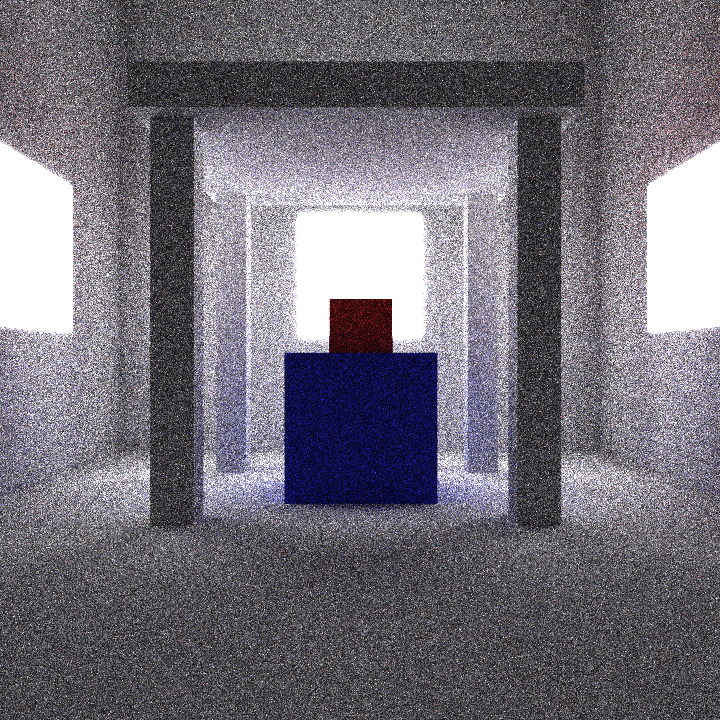
\includegraphics[width=\textwidth]{images/renders/shelter/default.png}   
  \subcaption{Default}
\endminipage\hspace{1em}
\minipage{0.45\textwidth}
  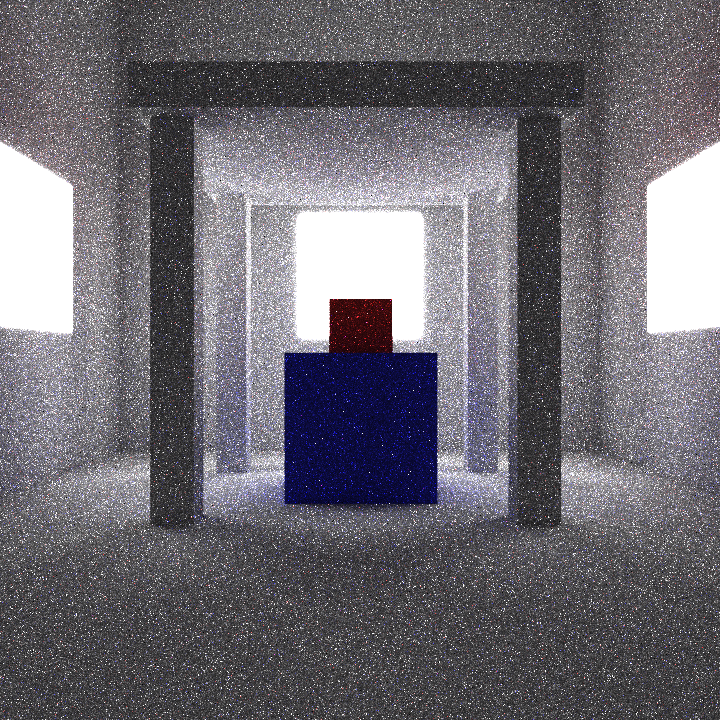
\includegraphics[width=\textwidth]{images/renders/shelter/sarsa.png}   
  \subcaption{Expected Sarsa}
\endminipage\hspace{1em}
\minipage{0.45\textwidth}
  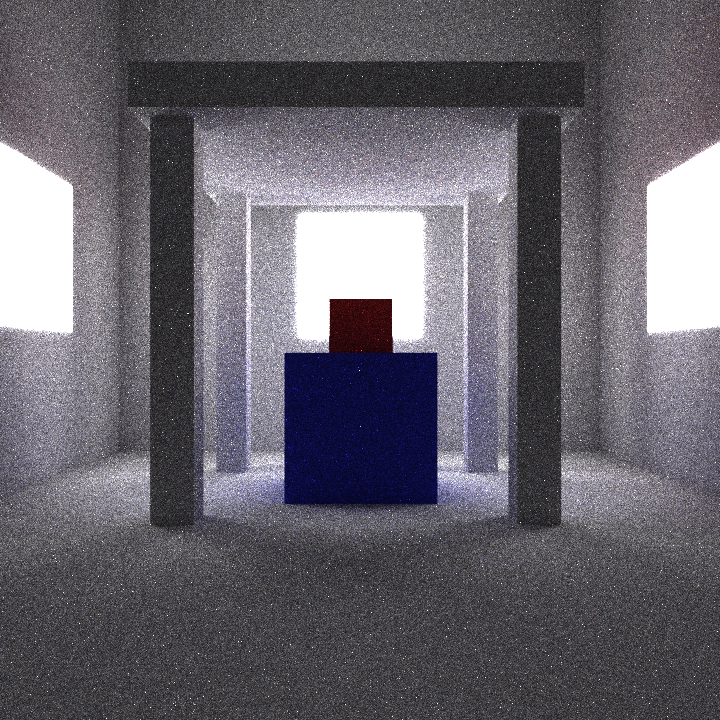
\includegraphics[width=\textwidth]{images/renders/shelter/nn.png}
  \subcaption{Neural-Q}
\endminipage
\caption{128 SPP renders for the Shelter scene.}
\label{fig:shelter}
\end{figure}



\begin{figure}[h]
\centering
\minipage{0.45\textwidth}
  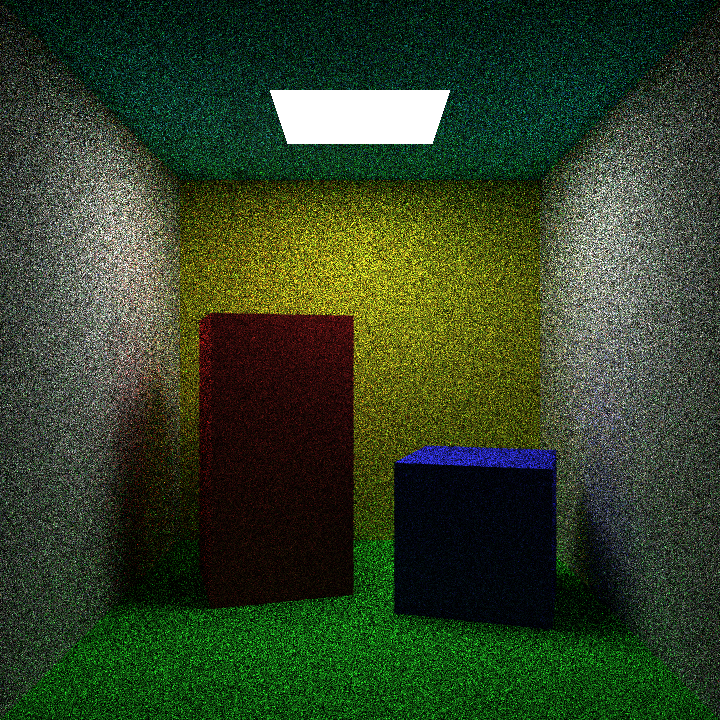
\includegraphics[width=\textwidth]{images/renders/cornell/default.png}   
  \subcaption{Default}
\endminipage\hspace{1em}
\minipage{0.45\textwidth}
  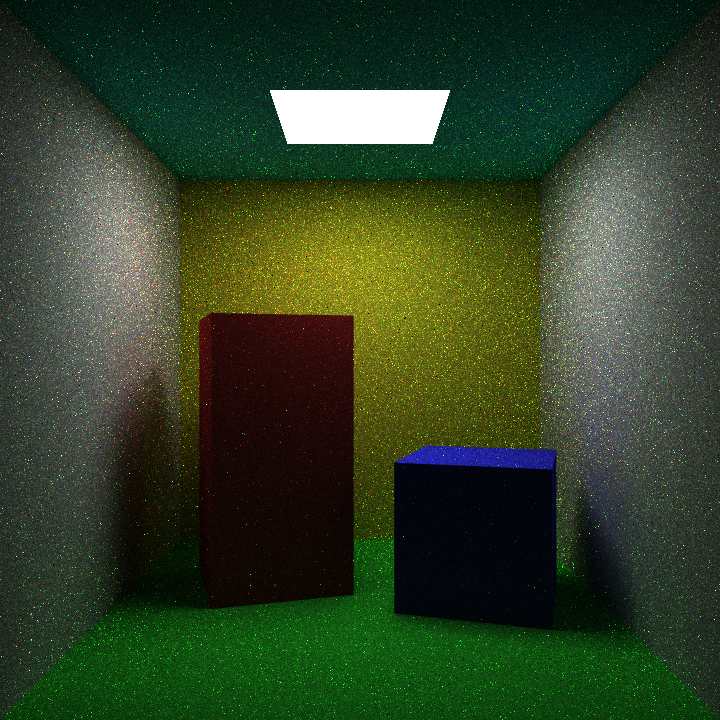
\includegraphics[width=\textwidth]{images/renders/cornell/sarsa.png}   
  \subcaption{Expected Sarsa}
\endminipage\hspace{1em}
\minipage{0.45\textwidth}
  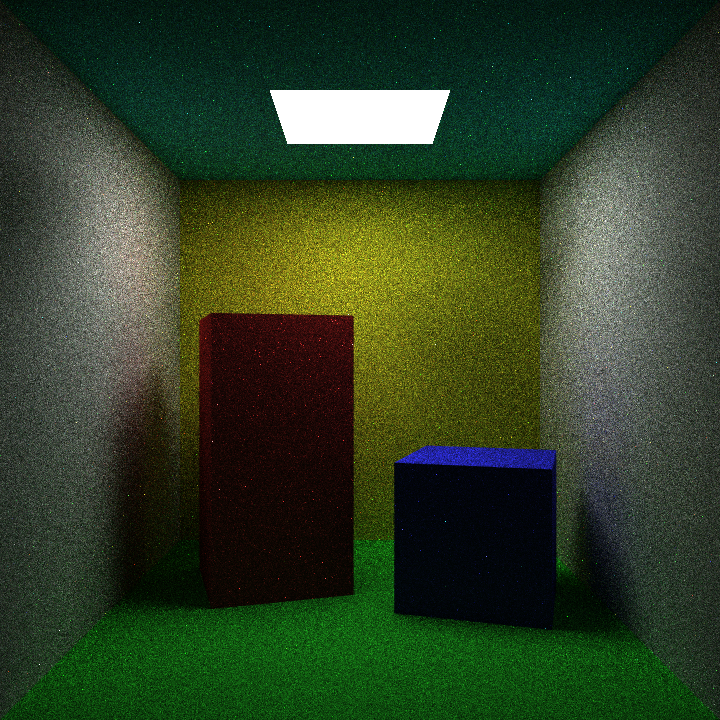
\includegraphics[width=\textwidth]{images/renders/cornell/nn.png}
  \subcaption{Neural-Q}
\endminipage
\caption{128 SPP renders for the Cornell Box scene.}
\label{fig:cornell}
\end{figure}



\begin{figure}[h]
\centering
\minipage{0.45\textwidth}
  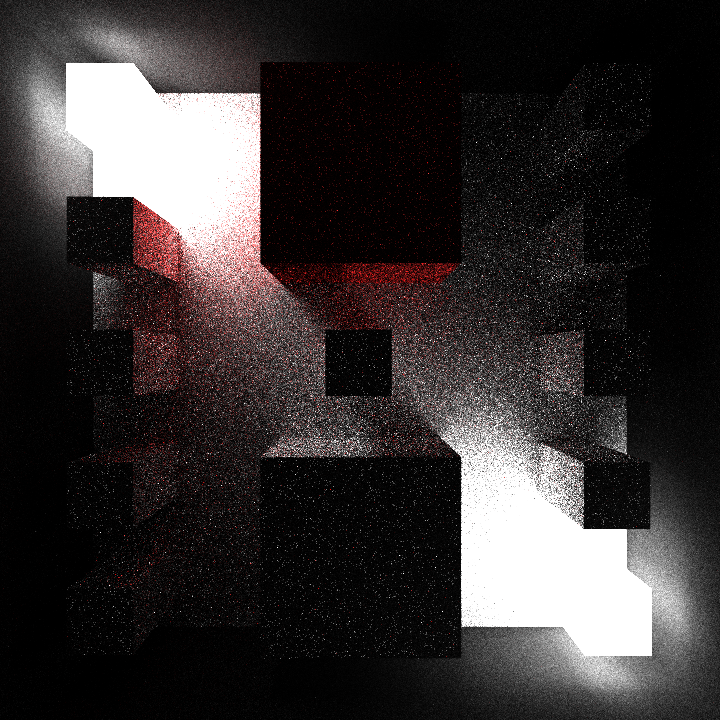
\includegraphics[width=\textwidth]{images/renders/complex_pillars/default.png}   
  \subcaption{Default}
\endminipage\hspace{1em}
\minipage{0.45\textwidth}
  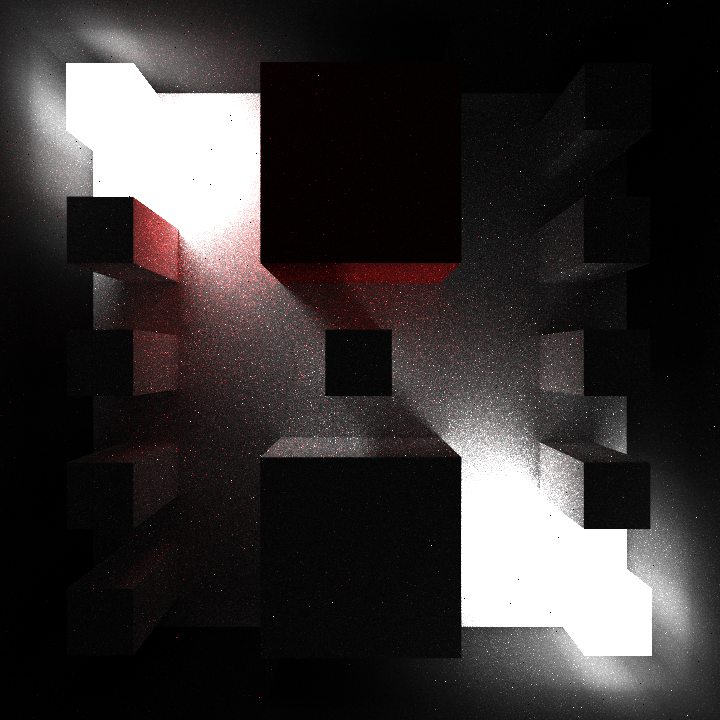
\includegraphics[width=\textwidth]{images/renders/complex_pillars/sarsa.png}   
  \subcaption{Expected Sarsa}
\endminipage\hspace{1em}
\minipage{0.45\textwidth}
  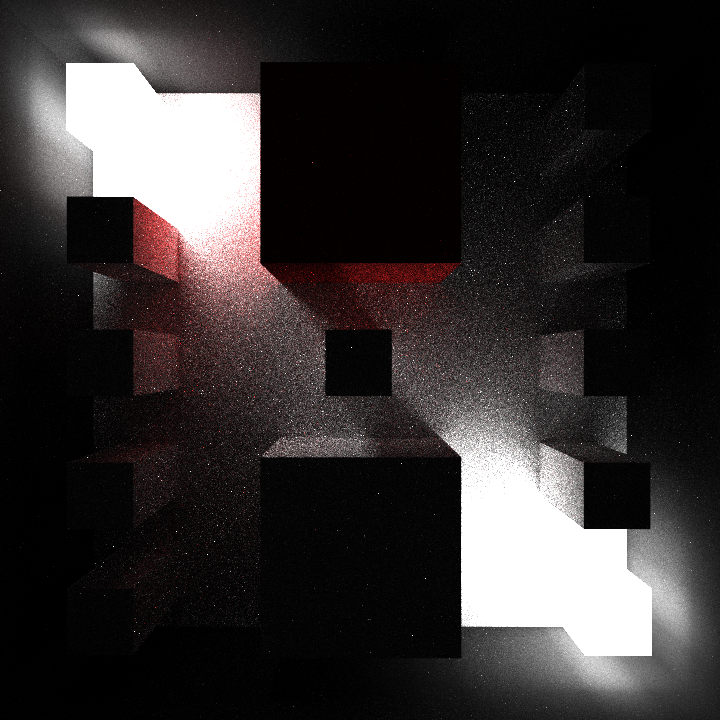
\includegraphics[width=\textwidth]{images/renders/complex_pillars/nn.png}
  \subcaption{Neural-Q}
\endminipage
\caption{128 SPP renders for the Complex Pillars scene.}
\label{fig:complex_light}
\end{figure}



\begin{figure}[h]
\centering
\minipage{0.45\textwidth}
  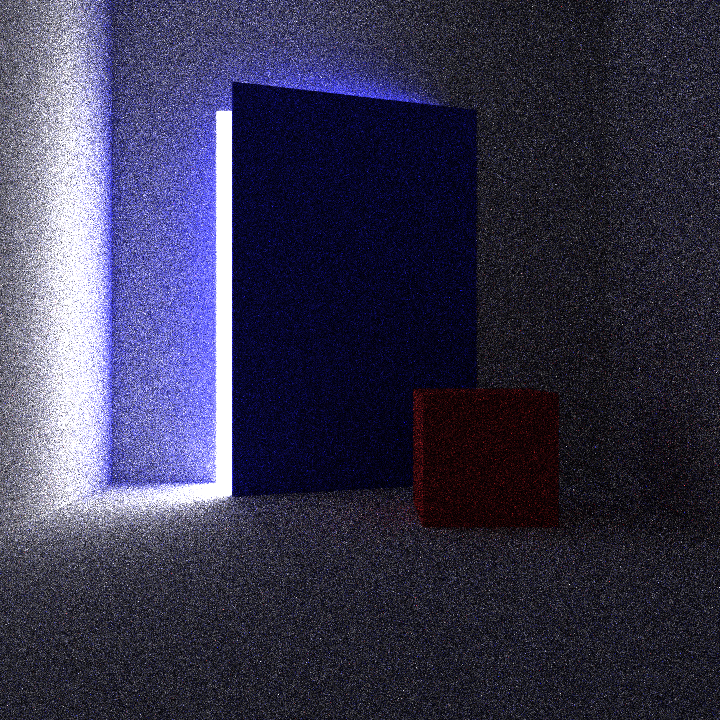
\includegraphics[width=\textwidth]{images/renders/door_room/default.png}   
  \subcaption{Default}
\endminipage\hspace{1em}
\minipage{0.45\textwidth}
  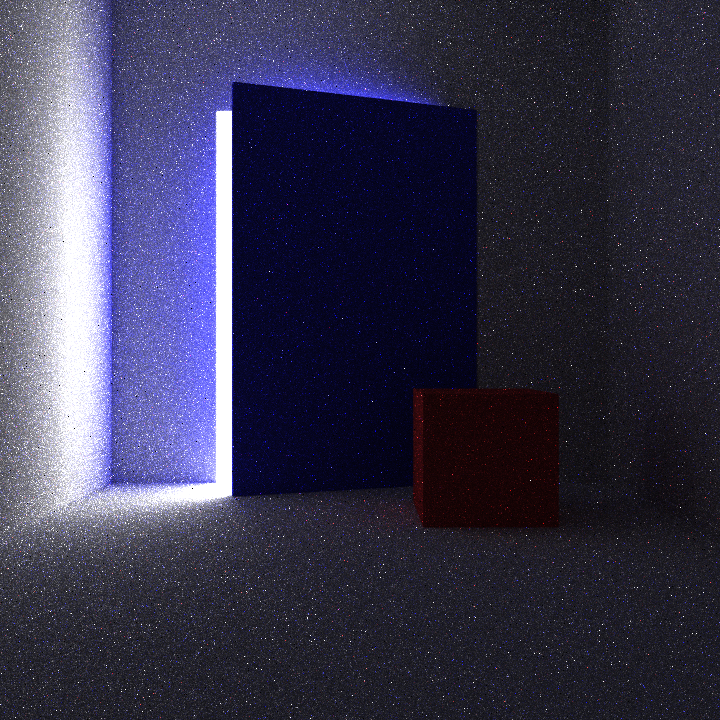
\includegraphics[width=\textwidth]{images/renders/door_room/sarsa.png}   
  \subcaption{Expected Sarsa}
\endminipage\hspace{1em}
\minipage{0.45\textwidth}
  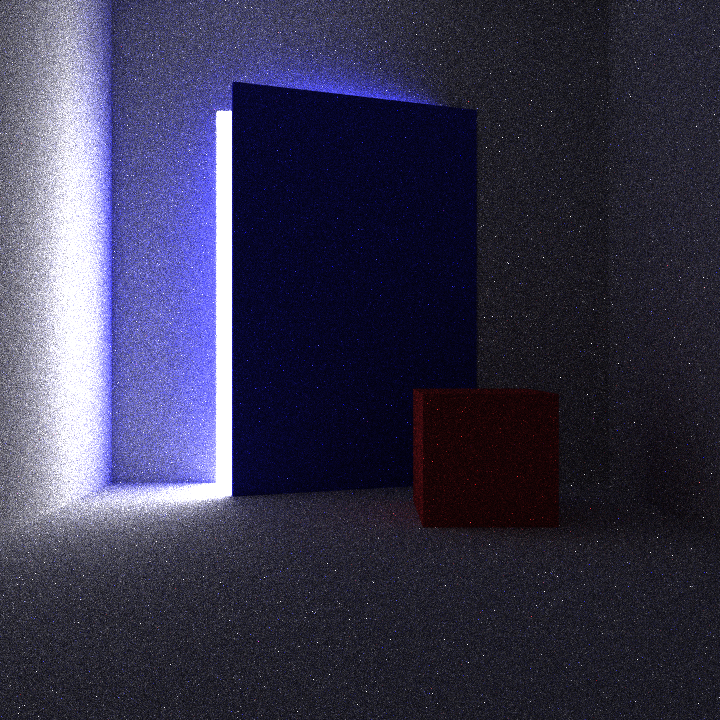
\includegraphics[width=\textwidth]{images/renders/door_room/nn.png}
  \subcaption{Neural-Q}
\endminipage
\caption{128 SPP renders for the Door Room scene.}
\label{fig:door_room}
\end{figure}

% =============================================================================

\end{document}
